\title{Study Guide for Midterm 1}
\author{Dr. Jordan Hanson - Whittier College Dept. of Physics and Astronomy}
\date{\today}
\documentclass[10pt]{article}
\usepackage[a4paper, total={18cm, 27cm}]{geometry}
\usepackage{outlines}
\usepackage{graphicx}
\begin{document}
\maketitle

\section{Chapter 1 - Introductory Concepts}

\begin{enumerate}
\item Consider Fig. \ref{fig:timing1}. (a) If the clock frequency is 10 MHz, what is the period?  (b) What is the length of time in the waveform? (c) What is the length of the pulse in channel $D0$?
\begin{figure}[ht]
\centering
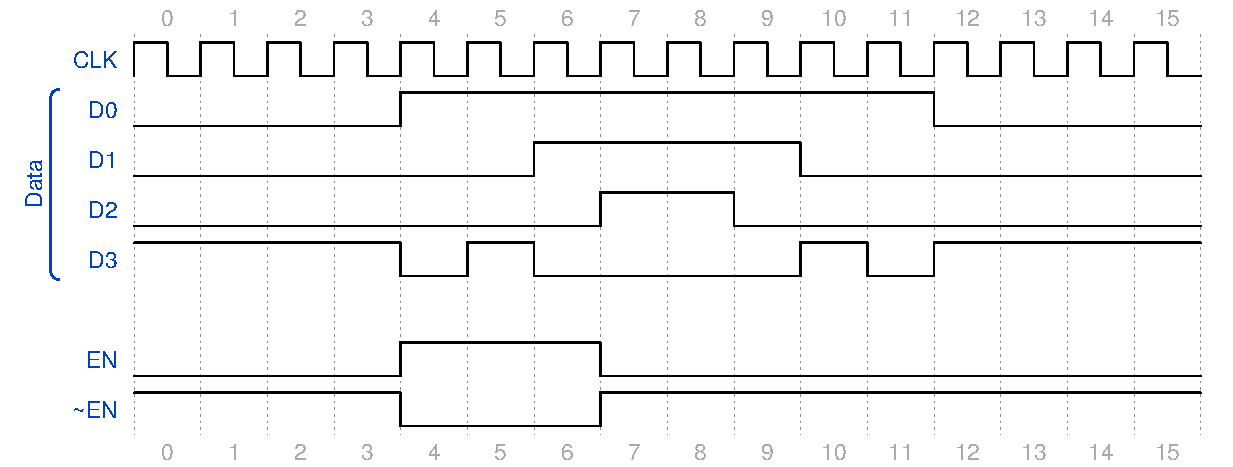
\includegraphics[width=0.9\textwidth]{timingExample1.pdf}
\caption{\label{fig:timing1}}
\end{figure}
\end{enumerate}

\section{Chapter 2}

\begin{enumerate}
\item \textbf{Scaling problem}: 
\end{enumerate}

\section{Chapter 3}

\begin{enumerate}
\item \textbf{Scaling problem}: 
\end{enumerate}

\section{Chapter 4}

\begin{enumerate}
\item \textbf{Scaling problem}: 
\end{enumerate}

\section{Chapter 5}

\begin{enumerate}
\item \textbf{Scaling problem}: 
\end{enumerate}

\end{document}